\section{Franck-Hertz-Versuch}\label{sec:franck-hertz}
Der Franck-Hertz-Versuch hat historisch maßgeblich zur Entwicklung 
der Quantenmechanik beigetragen und das damals von Niels Bohr vorgestellte 
Atommodell gestützt. Hierbei werden in einer Röhre Elektronen zu einer Anode hin 
beschleunigt und erzeugen einen messbaren 
Strom. Besitzen diese genügend kinetische Energie, so können 
diese inelastisch mit den Quecksilberatomen in dem Röhrengas stoßen, 
wobei der Energieübertrag zur Anregung atomarer Übergänge genutzt wird. 
Aufgrund der verringerten kinetischen Energie der beschleunigten Elektronen 
kommt es zu einem Stromeinbruch. Die dabei entstehende Spannungskurve wird 
wie in \cref{fig:franck-hertz-spannungskurve} erwartet. Die Stöße der Elektronen 
mit den Atomen ist ein statistischer Prozess. Ebenso unterliegt die Elektronengeschwindigkeit
einer Maxwell-Boltzmann-Verteilung, weshalb keine scharfen Maxima 
bei den entsprechenden Beschleunigungsspannungen erwartet werden, sondern 
normalverteilte Kurven.

Aus der Differenz den Abständen der Maxima kann somit die 
Energie des Übergangs bestimmt werden. Primär kann 
aufgrund des deutlich höheren Wirkungsquerschnittes der Übergang
${}6^1\mathrm S_0\rightarrow 6^3\mathrm P_1$ betrachtet werden. Der Wirkungsquerschnitt ist 
hierbei antiproportional zur freien Weglänge des Gases korreliert. 


\begin{figure}[h]
    \centering
    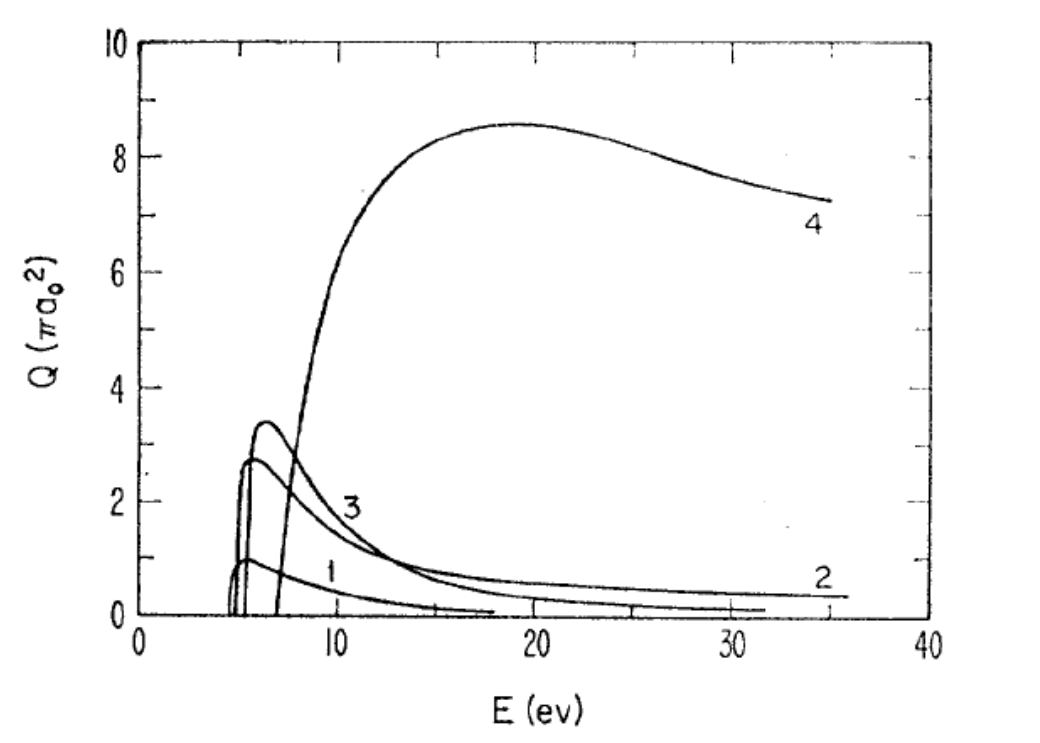
\includegraphics[width=0.6\linewidth]{../figs/querschnitt}
    \caption{Totale Wirkungsquerschnitte von \bf 1: $6^1\mathrm S_0\rightarrow 6^3\mathrm P_0$,
    \bf 2: $6^1\mathrm S_0\rightarrow 6^3\mathrm P_1$, 
    \bf 3: $6^1\mathrm S_0\rightarrow 6^3\mathrm P_2$,\\
    \bf 4: $6^1\mathrm S_0\rightarrow 6^1\mathrm P_1$ \cite{skript}}
    \label{fig:wirkungsquerschnitte}
\end{figure}

\subsection{Aufbau und Durchführung}
Um zunächst in einem Quecksilbergas freie Ladungsträger zu erzeugen, wird mit einer 
Heizspannung $U_\mathrm h$ ein Glühdraht erwärmt. In \cref{fig:schaltbild_franck_hertz} 
entspricht dies der Kathode K. Die Elektronen werden mit einer angelegten Beschleunigungsspannung
$U_\mathrm B$ zu einem Gitter G beschleunigt. 
Zwischen Gitter G und Anode A wird eine zusätzliche Gegenspannung $U_G$ angelegt, die Elektronen 
abbremst. Diese beschränkt die kinetische Energie der durch das Gitter kommenden
Elektronen nach unten und verringert so die an der Anode auftreffende Elektronenzahl.
Die Spannungskurve wird viermal bei unterschiedlichen Gegenspannungen und konstanter Temperatur 
gemessen und anschließend viermal bei gleichbleibender Gegenspannung und variabler 
Temperatur.

\begin{figure}[htb]
    \centering
    \begin{minipage}{.45\linewidth}
        \centering
        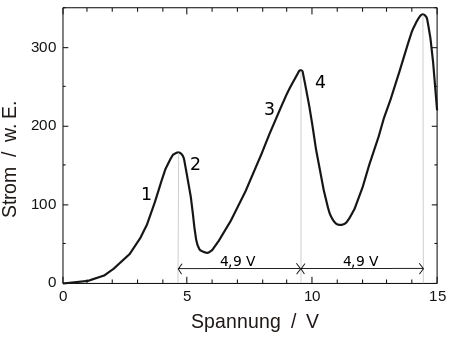
\includegraphics[width=\linewidth]{../figs/Franck-Hertz_spannungskurve}
        \caption{Franck-Hertz: Spannungskurve \cite{wiki:franck-hertz}}
        \label{fig:franck-hertz-spannungskurve}
    \end{minipage}
    \hspace{.5cm}
    \begin{minipage}{.45\linewidth}
        \centering
        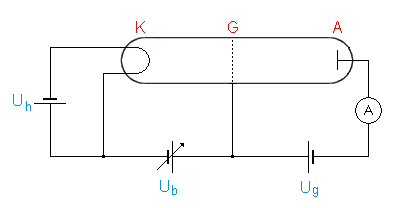
\includegraphics[width=\linewidth]{../figs/Schaltbild_Franck_Hertz_Versuch}
        \caption{Schaltbild Franck Hertz Versuche \cite{wiki:franck-hertz}}
        \label{fig:schaltbild_franck_hertz}
    \end{minipage}
\end{figure}

\subsection{Auswertung}
Die Unsicherheiten werden nach Herstellerangaben auf $\pm 1\%$ inklusive $\pm 0.5\%$ 
des Messbereiches gelegt. Der Messbereich beim genutzten Sensor ist variabel 
und wurde automatisch gesteuert, weshalb nur vermutet werden kann, dass dieser 
bei steigender Spannung immer auf den nächsten höheren Bereich umgestiegen ist. Die Fehler
wurden auf diese Weise für die Messung des Anodenstroms und Beschleunigungsspannung berechnet, wobei
zu beachten ist, dass kein eigentlicher Strom, sondern die dazu proportionale Spannung gemessen wurde.
Die Skalierung ist für die Auswertung jedoch nicht weiter wichtig. 

\begin{figure}[htb]
    \centering
    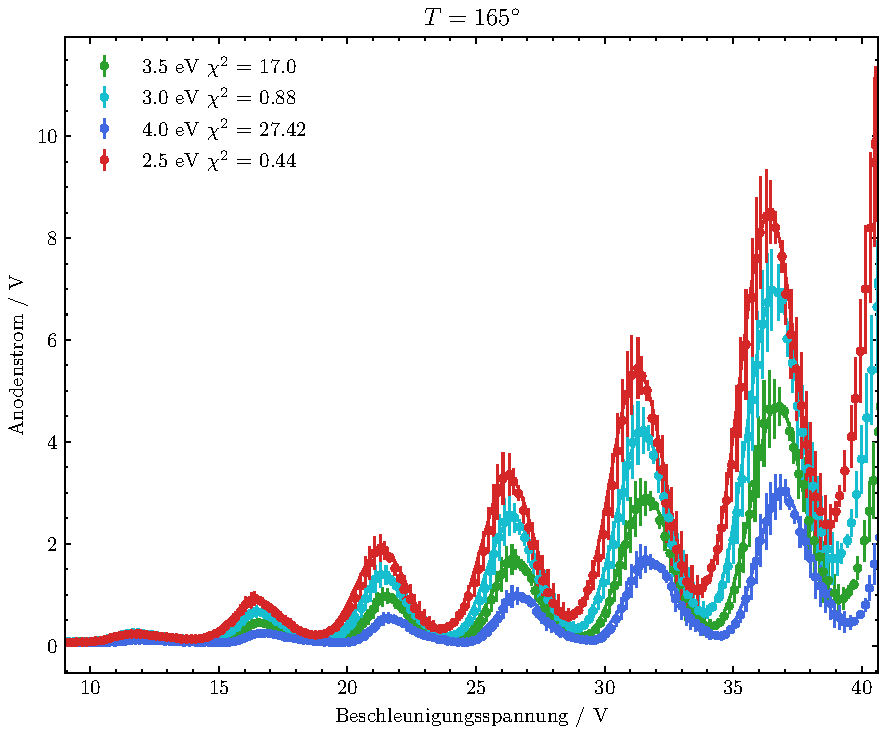
\includegraphics[width=0.6\linewidth]{../figs/franck-hertz_gegenspannung}
    \caption{Spannungskurve in Abhängigkeit der Gegenspannung bei \SI{165}{\celsius}}
    \label{fig:gegenspannung}
\end{figure}

\subsubsection{Abhängigkeit der Gegenspannung}\label{sec:franck-hertz-gegen}
Die Messdaten der Spannungskurven bei variabler Gegenspannung sind in 
\cref{fig:gegenspannung} grafisch dargestellt. An die Daten können Gauß-Kurven
angepasst werden. Die Parameter der Anpassung sind in \cref{tab:gegenspannung}
aufgezeigt. Das $\chi^2$ für die Anpassungen ist liegt dabei eine Größenordnung zu
hoch, da aber diese Maß der Güte nur die Fehler der y-Achse betrachtet und 
hier die Fehler in x-Richtung deutlich überwiegen, kann die Güte 
nicht die Anpassung richtig einschätzen. Visuell kann behauptet werden,
dass die Messdaten hier sehr gut beschrieben werden.

Zu Sehen ist, dass für größere Gegenspannungen 
die Maxima kleiner werden und leicht zu höheren Spannungen verschoben werden. 
Dies entspricht der Erwartung, dass bei höheren Gegenspannungen weniger 
Elektronen in den Bereich hinter das Gitter driften können.

Die Breite der Kurven nimmt dabei leicht ab, was jedoch im Fehlerbereich liegt.

Für Alle Gegenspannungen liegt die durchschnittliche Übergangsenergie im $1\sigma$-Bereich 
zum Literaturwert des Übergangs.

\subsubsection{Abhängigkeit der Temperatur}
Die Messdaten der Spannungskurven bei Variation der Temperatur 
sind in \cref{fig:temperatur} grafisch dargestellt und die Anpassparameter 
tabellarisch in \cref{tab:temperatur}. Die Güte der Anpassungskurven ist 
vergleichbar wie in \cref{sec:franck-hertz-gegen}. Auch hier ist erkennbar, dass 
bei steigender Temperatur die Maxima leicht zu höheren Spannungen hin verschoben 
werden mit gedämpften Amplituden und leicht erhöhten Breiten. Nach \cite{skript}
ist die Temperatur durch die Relation 
\begin{equation*}
    \log p = \num{10.55}-\frac{3333}{T}-\num{0.85}\log T
\end{equation*}
mit dem Druck korreliert. Diese Korrelation ist in \cref{fig:druck_temp} dargestellt. Wie zu 
erkennen ist, variiert in dem Bereich über der Raumtemperatur der Druck stark. Mit 
höherem Druck nimm ebenso die Anzahl der Stöße zu, weshalb weniger Elektronen die Gegenspannung
überwinden können und dadurch die Amplitude der Kurven sinkt. Die Driftgeschwindigket 
der Elektronen ist antiproportional zur freien Weglänge, weshalb bei erhöhter Temperatur 
eine höhere Beschleunigungsspannung zur Stoßanregung benötigt wird. Dies erklärt auch 
die leichte Verschiebung der Maxima. Zu Erkennen ist ebenfalls, dass für die ersten 
vier Maxima die Breite leicht zunimmt (bei dem ersten ist die Zunahme wieder sehr stark), 
für die letzten Beiden jedoch konstant bleibt. 
Eine offensichtliche Erklärung hierfür lässt sich nicht eindeutig finden. Es besteht 
die Möglichkeit, dass für zu kleine Spannungen die Energie der Elektronen sich in
dem Bereich befindet, wo nach \cref{fig:wirkungsquerschnitte} die Wirkungsquerschnitte
der zwei niedrigsten Übergänge ähnlich groß sind, weshalb sich hier die 
Kurven der Anregung überlagern.

Die Energien der Übergänge sind in \cref{tab:temperatur} aufgetragen mit dem Mittelwert 
in der letzten Spalte. Zu Erkennen ist dabei, dass bei der kleinsten Temperatur noch eine 
Energie von \SI{4.8(3)}{\electronvolt} gemessen wurde, bei höheren Temperaturen 
sinkt diese auf \SI{4.6(3)}{\electronvolt} ab. Dies lässt sich mit \cref{fig:wirkungsquerschnitte}
erklären. Bei zu hohen Temperaturen wird die freie Weglänge der Elektronen so stark begrenzt, 
dass nur noch das niedrigste Energieniveau angeregt werden kann. Bei zu kleinen Temperaturen 
würde hingegen der Übergang $6^1\mathrm S_0\rightarrow 6^1\mathrm P_1$ überwiegen. Der Bereich,
in dem der Streuquerschnitt des hier untersuchten Übergangs überwiegt, ist klein, weshalb 
das Temperaturintervall ebenso klein gewählt werden musste.

\begin{figure}[htb]
    \centering
    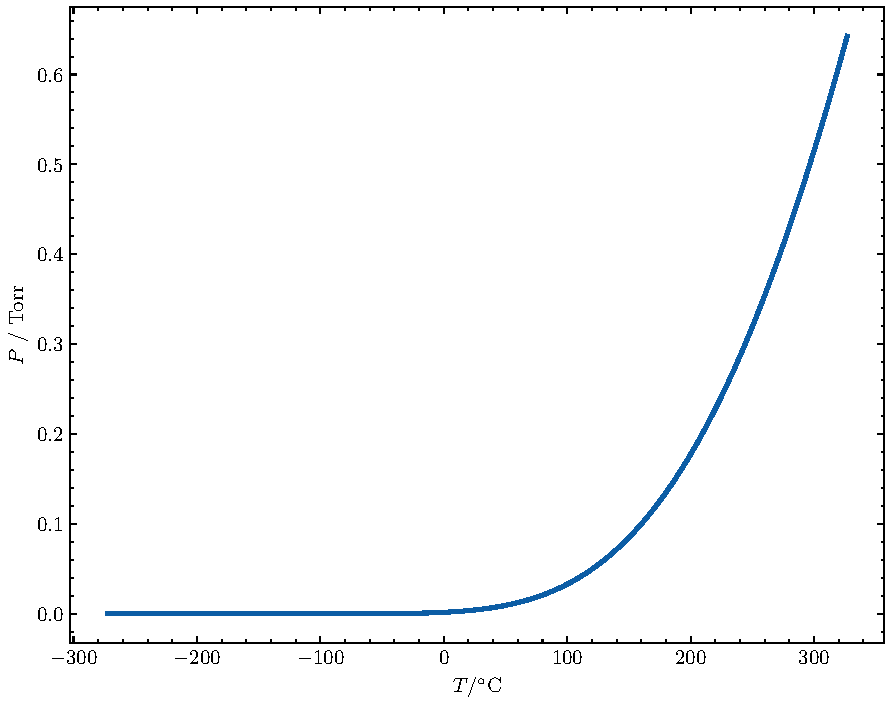
\includegraphics[width=.5\linewidth]{../figs/druck_temp}
    \caption{Temperaturabhängigkeit des Drucks}
    \label{fig:druck_temp}
\end{figure}


\begin{figure}[htb]
    \centering
    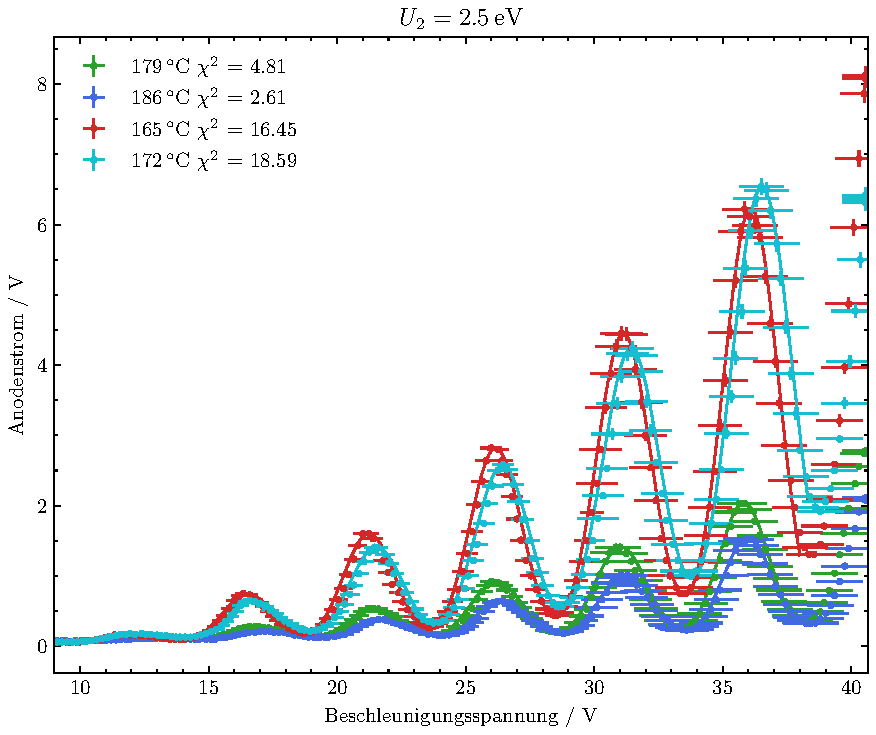
\includegraphics[width=0.6\linewidth]{../figs/franck-hertz_temperatur}
    \caption{Spannungskurve in Abhängigkeit der Temperatur bei einer Gegenspannung von \SI{2.5}{\volt}}
    \label{fig:temperatur}
\end{figure}

\begin{table}[htb]
   \centering
\caption{Anpassparameter der Spannungskurve für verschiedene Gegenspannungen}
\begin{tabular}{c|cc|cc|cc|cc}
\hline & \multicolumn{2}{|c}{\SI{2.5}{\volt}} & \multicolumn{2}{|c}{\SI{3.0}{\volt}} & \multicolumn{2}{|c}{\SI{3.5}{\volt}} & \multicolumn{2}{|c}{\SI{4.0}{\volt}}\\

\hline
Maximum & $x_0$ / \unit{\volt} & $\sigma$ / \unit{\volt} & $x_0$ / \unit{\volt} & $\sigma$ / \unit{\volt} & $x_0$ / \unit{\volt} & $\sigma$ / \unit{\volt} & $x_0$ / \unit{\volt} & $\sigma$ / \unit{\volt} \\ 
\hline
$\num{1}$ & $\num{11.97\pm 0.03}$ & $\num{1.35\pm 0.03}$ & $\num{11.96\pm 0.03}$ & $\num{1.28\pm 0.03}$ & $\num{12.10\pm 0.04}$ & $\num{1.49\pm 0.05}$ & $\num{12.17\pm 0.07}$ & $\num{1.84\pm 0.11}$ \\
$\num{2}$ & $\num{16.52\pm 0.03}$ & $\num{1.031\pm 0.016}$ & $\num{16.64\pm 0.03}$ & $\num{1.00\pm 0.02}$ & $\num{16.81\pm 0.04}$ & $\num{0.98\pm 0.03}$ & $\num{17.04\pm 0.05}$ & $\num{1.01\pm 0.04}$ \\
$\num{3}$ & $\num{21.32\pm 0.03}$ & $\num{1.023\pm 0.016}$ & $\num{21.47\pm 0.03}$ & $\num{0.999\pm 0.018}$ & $\num{21.61\pm 0.04}$ & $\num{0.96\pm 0.03}$ & $\num{21.77\pm 0.04}$ & $\num{0.96\pm 0.03}$ \\
$\num{4}$ & $\num{26.26\pm 0.03}$ & $\num{1.031\pm 0.019}$ & $\num{26.45\pm 0.03}$ & $\num{0.995\pm 0.019}$ & $\num{26.56\pm 0.04}$ & $\num{0.97\pm 0.03}$ & $\num{26.74\pm 0.05}$ & $\num{0.97\pm 0.03}$ \\
$\num{5}$ & $\num{31.29\pm 0.05}$ & $\num{1.10\pm 0.03}$ & $\num{31.50\pm 0.06}$ & $\num{1.04\pm 0.04}$ & $\num{31.66\pm 0.07}$ & $\num{1.02\pm 0.04}$ & $\num{31.85\pm 0.08}$ & $\num{0.97\pm 0.05}$ \\
$\num{6}$ & $\num{36.40\pm 0.07}$ & $\num{1.15\pm 0.06}$ & $\num{36.61\pm 0.09}$ & $\num{1.09\pm 0.06}$ & $\num{36.72\pm 0.11}$ & $\num{1.03\pm 0.07}$ & $\num{36.92\pm 0.13}$ & $\num{0.97\pm 0.09}$ \\
\hline\end{tabular}
\label{tab:gegenspannung}
\end{table}\begin{table}[htb]
   \centering
\caption{Anpassparameter der Spannungskurve für verschiedene Temperaturen}
\begin{tabular}{c|cc|cc|cc|cc}
\hline & \multicolumn{2}{|c}{\SI{165}{\celsius}} & \multicolumn{2}{|c}{\SI{172}{\celsius}} & \multicolumn{2}{|c}{\SI{179}{\celsius}} & \multicolumn{2}{|c}{\SI{186}{\celsius}}\\

\hline
Maximum & $x_0$ / \unit{\volt} & $\sigma$ / \unit{\volt} & $x_0$ / \unit{\volt} & $\sigma$ / \unit{\volt} & $x_0$ / \unit{\volt} & $\sigma$ / \unit{\volt} & $x_0$ / \unit{\volt} & $\sigma$ / \unit{\volt} \\ 
\hline
$\num{1}$ & $\num{12.00\pm 0.03}$ & $\num{1.43\pm 0.04}$ & $\num{12.33\pm 0.04}$ & $\num{1.57\pm 0.04}$ & $\num{12.42\pm 0.06}$ & $\num{1.99\pm 0.08}$ & $\num{12.79\pm 0.12}$ & $\num{3.0\pm 0.3}$ \\
$\num{2}$ & $\num{16.55\pm 0.03}$ & $\num{1.023\pm 0.016}$ & $\num{16.82\pm 0.03}$ & $\num{1.109\pm 0.018}$ & $\num{17.05\pm 0.03}$ & $\num{1.21\pm 0.03}$ & $\num{17.48\pm 0.04}$ & $\num{1.21\pm 0.05}$ \\
$\num{3}$ & $\num{21.24\pm 0.03}$ & $\num{1.030\pm 0.014}$ & $\num{21.53\pm 0.03}$ & $\num{1.094\pm 0.016}$ & $\num{21.51\pm 0.03}$ & $\num{1.15\pm 0.02}$ & $\num{21.80\pm 0.03}$ & $\num{1.25\pm 0.03}$ \\
$\num{4}$ & $\num{26.17\pm 0.03}$ & $\num{1.021\pm 0.016}$ & $\num{26.43\pm 0.03}$ & $\num{1.083\pm 0.016}$ & $\num{26.21\pm 0.03}$ & $\num{1.085\pm 0.017}$ & $\num{26.45\pm 0.03}$ & $\num{1.16\pm 0.02}$ \\
$\num{5}$ & $\num{31.15\pm 0.05}$ & $\num{1.06\pm 0.03}$ & $\num{31.43\pm 0.05}$ & $\num{1.14\pm 0.03}$ & $\num{31.04\pm 0.05}$ & $\num{1.06\pm 0.03}$ & $\num{31.24\pm 0.04}$ & $\num{1.11\pm 0.03}$ \\
$\num{6}$ & $\num{36.09\pm 0.06}$ & $\num{1.08\pm 0.04}$ & $\num{36.52\pm 0.07}$ & $\num{1.19\pm 0.05}$ & $\num{35.82\pm 0.06}$ & $\num{1.01\pm 0.05}$ & $\num{35.98\pm 0.07}$ & $\num{1.03\pm 0.05}$ \\
\hline\end{tabular}
\label{tab:temperatur}
\end{table}

\begin{table}[htb]
   \centering
\caption{Übergangsenergien bei verschiedenen Gegenspannungen}
\begin{tabular}{c c c c c}
\hline Maximum & \SI{2.5}{\volt} & \SI{3.0}{\volt} & \SI{3.5}{\volt} & \SI{4.0}{\volt} \\ 
\hline
$\num{1}$ & $\num{4.55\pm 0.04}$ & $\num{4.68\pm 0.04}$ & $\num{4.71\pm 0.05}$ & $\num{4.88\pm 0.09}$ \\
$\num{2}$ & $\num{4.80\pm 0.04}$ & $\num{4.83\pm 0.04}$ & $\num{4.79\pm 0.05}$ & $\num{4.73\pm 0.06}$ \\
$\num{3}$ & $\num{4.94\pm 0.04}$ & $\num{4.98\pm 0.05}$ & $\num{4.96\pm 0.06}$ & $\num{4.97\pm 0.06}$ \\
$\num{4}$ & $\num{5.03\pm 0.06}$ & $\num{5.05\pm 0.07}$ & $\num{5.10\pm 0.08}$ & $\num{5.11\pm 0.09}$ \\
$\num{5}$ & $\num{5.12\pm 0.09}$ & $\num{5.12\pm 0.11}$ & $\num{5.06\pm 0.13}$ & $\num{5.07\pm 0.15}$ \\
$\langle E\rangle$ & $\num{4.9\pm 0.3}$ & $\num{4.9\pm 0.3}$ & $\num{4.9\pm 0.3}$ & $\num{5.0\pm 0.3}$ \\
\hline\end{tabular}
\label{fig:energy_gegen}
\end{table}\begin{table}[htb]
   \centering
\caption{Übergangsenergien bei verschiedenen Temperaturen}
\begin{tabular}{c c c c c}
\hline Maximum & \SI{165}{\celsius} & \SI{172}{\celsius} & \SI{179}{\celsius} & \SI{186}{\celsius} \\ 
\hline
$\num{1}$ & $\num{4.54\pm 0.04}$ & $\num{4.50\pm 0.04}$ & $\num{4.63\pm 0.06}$ & $\num{4.69\pm 0.13}$ \\
$\num{2}$ & $\num{4.70\pm 0.03}$ & $\num{4.70\pm 0.04}$ & $\num{4.46\pm 0.04}$ & $\num{4.32\pm 0.04}$ \\
$\num{3}$ & $\num{4.93\pm 0.04}$ & $\num{4.91\pm 0.04}$ & $\num{4.70\pm 0.04}$ & $\num{4.65\pm 0.04}$ \\
$\num{4}$ & $\num{4.98\pm 0.05}$ & $\num{5.00\pm 0.05}$ & $\num{4.82\pm 0.05}$ & $\num{4.79\pm 0.05}$ \\
$\num{5}$ & $\num{4.95\pm 0.08}$ & $\num{5.09\pm 0.08}$ & $\num{4.78\pm 0.08}$ & $\num{4.73\pm 0.08}$ \\
$\langle E\rangle$ & $\num{4.8\pm 0.3}$ & $\num{4.8\pm 0.3}$ & $\num{4.7\pm 0.2}$ & $\num{4.6\pm 0.3}$ \\
\hline\end{tabular}
\label{fig:energy_temp}
\end{table}

